\section{Related Work}
%%%%%%%%%%%%%%%%%%%%%%%%%%%%%%%%%%%%
\begin{figure*}[t]
    \centering
    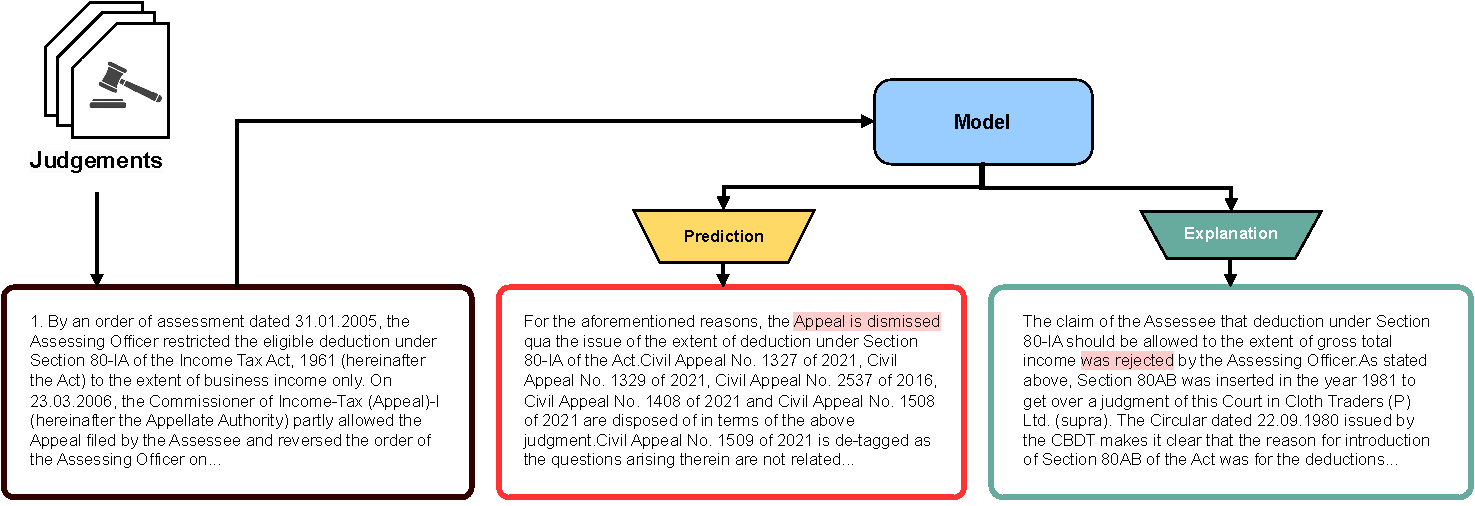
\includegraphics[width=\linewidth]{images/task_description_2.pdf}
    \caption{Illustration of the CJPE Task Framework.}
    \label{fig:task-framework}
\end{figure*}
%%%%%%%%%%%%%%%%%%%%%%%%%%%%%%%%%%%%
The field of Legal Natural Language Processing (NLP) has witnessed significant advancements, with researchers exploring a variety of complex tasks within the legal domain. A prominent area of focus has been Legal Judgment Prediction (LJP), where the goal is to predict the outcomes of legal cases based on their facts and contexts. Seminal works in this area include the contributions of \cite{zhong2020iteratively}, \cite{malik-etal-2021-ildc}, \cite{aletras2016predicting}, \cite{chen-etal-2019-charge} \cite{long2019automatic}, \cite{xu-etal-2020-distinguish} \cite{10.5555/3367471.3367609}, and \cite{chalkidis2019neural}. These studies have laid the groundwork for understanding the nuances involved in automating legal decision-making processes.

Another key area of research has been the application of Large Language Models (LLMs) in the legal field. The versatility of models such as GPT, BLOOM, FLAN-T5, and LlaMA has been demonstrated in various studies, including those by \cite{vats-etal-2023-llms} \cite{StatutoryReasoningGPT2023} and \cite{barExamGPT4}, highlighting their potential in tasks ranging from statutory reasoning to judgment prediction. However, challenges remain in terms of the acceptability and reliability of LLMs in high-stakes legal contexts. The LegalEval \cite{modi-etal-2023-semeval} workshop further exemplifies the diversity and complexity of legal NLP research, especially on legal judgment prediction and explanation.

Our research utilizes advanced Large Language Models and a comprehensive dataset to create a system that predicts and explains judicial outcomes, enhancing legal text processing and transparency. This work supports legal practitioners and the public, especially in complex systems like India's, and sets the stage for future AI advancements in legal technology.

